\chapter{Resultados}

Se mostrarán las pantallas que se obtuvieron al desarrollar la aplicación.

\begin{figure}[H]
	\begin{center}
		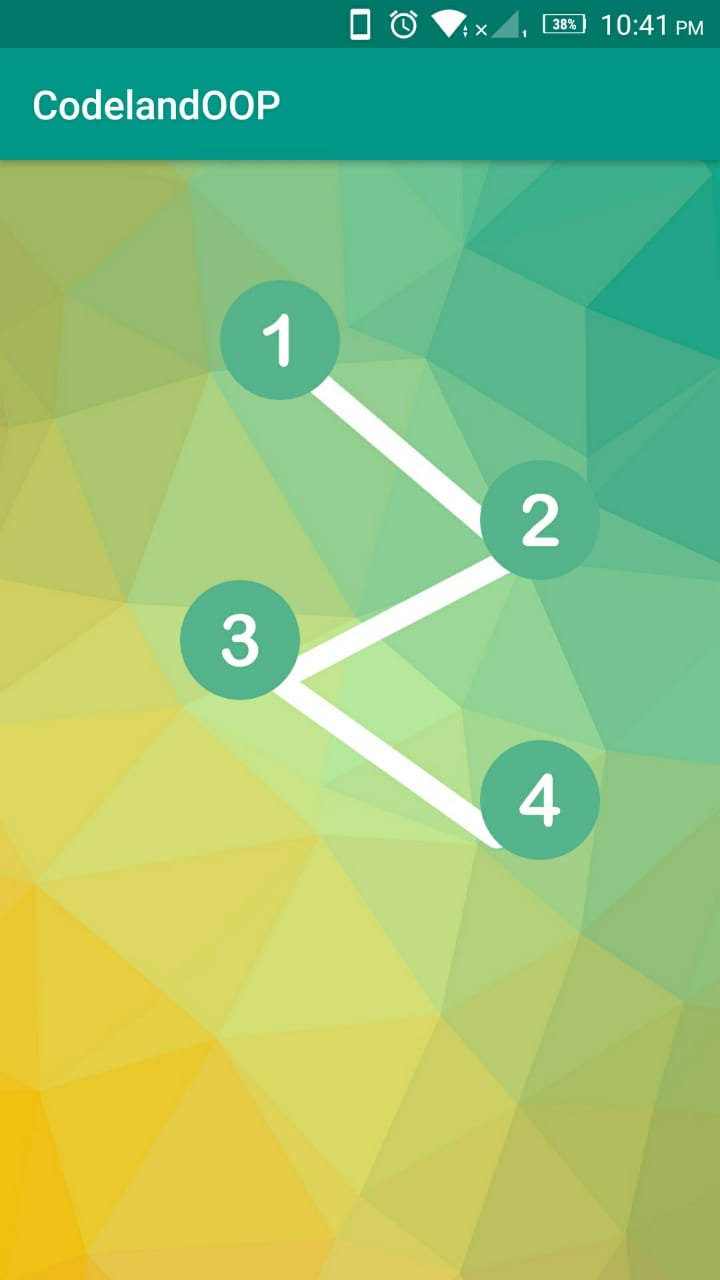
\includegraphics[scale=0.3]{img/ss1.jpg} 
		\caption{Pantalla de inicio donde se muestran las fases.}
		\label{fases}
	\end{center}
\end{figure}

\begin{figure}[H]
	\begin{center}
		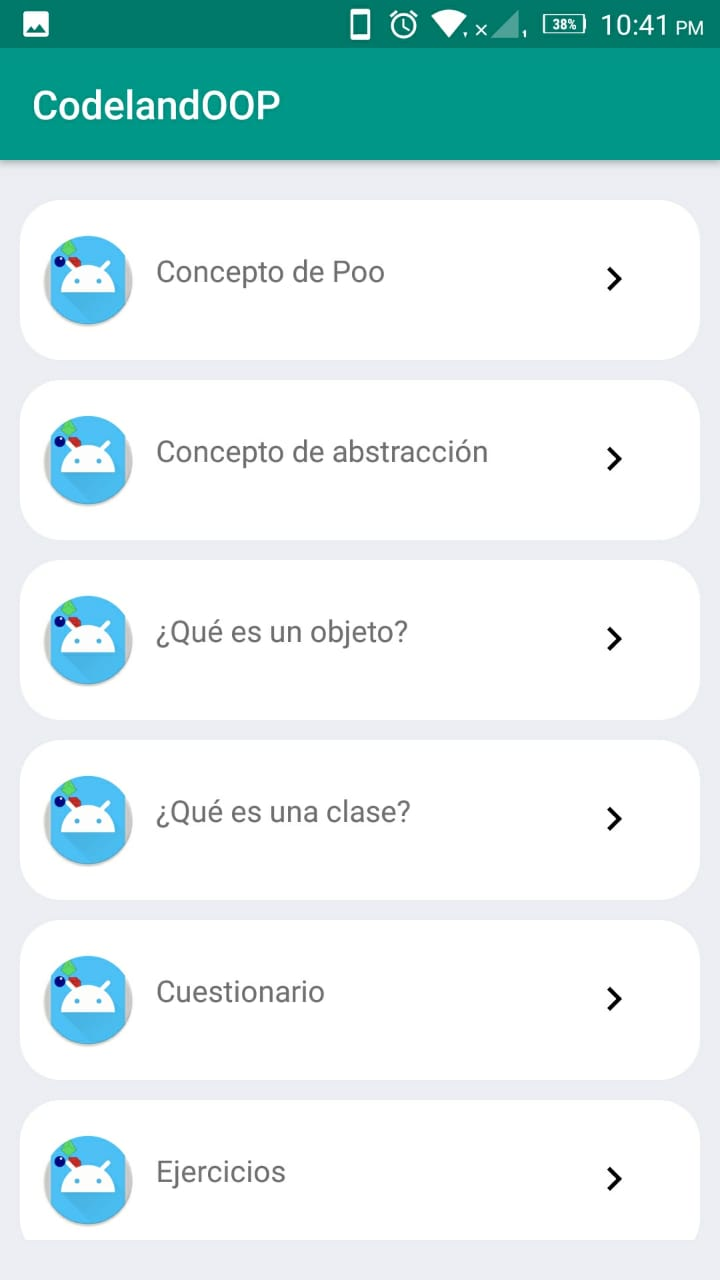
\includegraphics[scale=0.3]{img/ss2.jpg} 
		\caption{Pantalla de selección de los temas de cada fase.}
		\label{temas}
	\end{center}
\end{figure}
\section{Conclusiones Personales}
\textbf{Juan Antonio Ayola Cortés: }En conclusión debo decir que en verdad me a gustado mucho participar en este proyecto aprendi muchas cosas, ademas espero que en verdad se pueda aplicar y resolver nuestra problematica\\\newline
\textbf{Juan Daniel Soto Dimas: }En conclusión puedo decir que me di cuenta que la programación orientada a objetos es muy importante ya que todos los programas actualmente estan elaborados bajo este paradigma y es importante que los alumnos lo conoscan y no deserten por falta de conocimiento de este paradigma y lo apliquen en programas buenos.\\\newline
\textbf{Miguel Angel Vite Hernández:}Es muy Interesante participar en este proyecto ya que con este se puede reducir los altos índices de deserción que hay en los estudiantes de alguna ingenieria en informática o en sistemas\\\newline

\section{Conclusión General}
El el proyecto realizado se ha logrado desarrollar una aplicación para dispositivos móviles, capaz de mostrar y proporcionar información acerca del paradigma de programación orientada a objetos, enfocada a 3 distintos lenguajes(C Sharp,C++ y Java)ademas de tener cuestionarios y ejercicios como forma de evaluación.Ha logrado cumplir con todos los objetivos básicos que se habian propuesto \\\newline

En la introducción de este documento hablamos sobre cuáles son los objetivos que se desean lograr con este proyecto, y mencionamos que una parte importante que queremos solucionar era la tasa de abandono escolar universitario en el área de software,con nuestra aplicación esperamos apoyar al estudiante ofreciendo una manera lúdica de aprender o repasar la programación orientada a objetos, una parte importante a contemplar a futuro es la forma de hacer llegar nuestra aplicación a los estudiantes.\\\newline

La aplicación desarrollada ofrece una ventaja frente a otras que enfocan la informacion a un lenguaje específico, que no hacen uso de algun método de evaluación al usuario (tests o ejerciciós) ademas de tener la información mayormente en idioma ingles.\\\newline

La aplicación desarrollada tiene la posibilidad de crecer, es escalable en puntos como agregar mas información, nuevos temas o subtemas asi como enfocarlo a lenguajes nuevos, una idea futura es la implementación de juegos como una forma mas de evaluación y aprendizaje, ademas se propone mejorar la interfaz gráfica para aumentar la usabilidad del usuario y para un mayor alcance en la población, esta aplicación deberia de ser desarrollada para otras plataformas móviles.\\\newline

Finalmente, este proyecto ha demostrado que es viable, cuenta con disintas vias de publicación a la comunidad y de obtención de recurso económico, el resultado a sido satisfactorio gracias a que ha sido desarrollado empleando estandares y conocimientos de Ingenieria en Software, y esperamos impactar positivamente en los estudiantes implementando este proyecto.